\chapter{Background Theory}

\section{FREEDM DGI}

The FREEDM DGI is a smart grid operating system that organizes and coordinates power electronics and negotiates contracts to deliver power to devices and regions that cannot effectively facilitate their own need.

To accomplish this, the DGI software consists of a central component, the broker, which is responsible for presenting a communication interface and furnishing any common functionality needed by any algorithms used by the system. These algorithms are grouped into modules. These algorithms work in concert to move power from areas of excess supply to excess demand.

The initial work this document uses a version of the FREEDM DGI software with only one module: group management. Group management implements a leader election algorithm to discover which nodes are reachable in the cyber domain. A full system would feature additional modules, that provide additional functionality such as collecting a global snapshot, and a module which negotiates the migrations and gives commands to physical components. Additionally, a full implementation of the system is real-time which creates a maximum time before the system reacts to a change in the physical or cyber network.

\section{Broker Architecture}

The DGI software is designed around the broker architecture specification. Each core functionality of the system is implemented within a module which is provided access to core interfaces which deliver functionality such as scheduling requests, message passing, and a framework to manipulate physical devices, including those which exist only in simulation environments such as PSCAD\cite{PSCAD} and RSCAD\cite{RSCAD}.

The Broker provides a common message passing interface which all modules are allowed access to. This interface also provides the inter-module communication which delivers messages between software modules, effectively decoupling them outside of the requirement for them to be able to recognize messages addressed to them from other modules.

Several of the distributed algorithms used in the software require the use of ordered communication channels. To achieve this, FREEDM provides a reliable ordered communication protocol (The sequenced reliable connection or SRC) to the modules, as well as a ``best effort'' protocol (The sequenced unreliable connection or SUC) which is also FIFO (first in, first out), but provides limited delivery guarantees.

We elected to design and implement our own simple message delivery schemes in order to avoid complexities introduced by using TCP in our system. During development, it was observed that constructing a TCP connection to a node that had failed or was unreachable took a considerable amount of time. We elected to use UDP packets which do not have those issues, since the protocol is connectionless. UDP also allows development of protocols with various properties to evaluate which properties are desirable. To accomplish this lightweight protocols which are best effort oriented were implemented to deliver messages as quickly as possible within the requirements.

\subsection{Sequenced Reliable Connection.}

The sequenced reliable connection is a modified send and wait protocol with the 
ability to stop resending messages and move on to the next one in the queue if 
the message delivery time exceeds some timeout. When designing this scheme we
wanted to achieve several criteria:

\begin{itemize}
\item Messages must be delivered in order - Some distributed algorithms rely on 
the assumption that the underlying message channel is FIFO.
\item Messages can become irrelevant - Some messages may only have a short 
period in which they are worth sending. Outside of that time period, they 
should be considered inconsequential and should be skipped. To achieve this, we 
have added message expiration times. After a certain amount of time has passed, 
the sender will no longer attempt to write that message to the channel. 
Instead, he will proceed to the next unexpired message and attach a ``kill'' 
value to the message being sent, with the number of the last message the sender 
knows the receiver accepted.
\item As much effort as possible should be applied to deliver a message while 
it is still relevant.
\end{itemize}

There one adjustable parameter, the resend time, which controls how often the 
system would attempt to deliver a message it hadn't yet received an 
acknowledgement for. To further explain the characteristics of the protocol, 
the psuedocode is included in Appendix REF

Note that the $Resend()$ function is periodically called to attempt to redeliver
lost messages to the receiver. 

\subsection{Sequenced Unreliable Connection.}

The SUC protocol is simply a best effort protocol: it employs a sliding window 
to try to deliver messages as quickly as possible. A window size is decided, 
and then at any given time, the sender can have up to that many messages in the 
channel, awaiting acknowledgement. The receiver will look for increasing 
sequence numbers, and disregard any message that is of a lower sequence number 
than is expected. The purpose of this protocol is to implement a bare minimum: 
messages are accepted in the order they are sent.

Like the SRC protocol, the SUC protocol's resend time can be adjusted. 
Additionally, the window size is also configurable, but was left unchanged for 
the tests presented in this work. The psuedocode is included included in Appendix REF

\section{Group Management Algorithm}

Our software uses a leader election algorithm, ``Invitation Election 
Algorithm'' written by Garcia-Molina in \cite{INVITATIONELECTION}. 
His algorithm provides a robust election procedure which allows for transient 
partitions. Transient partitions are formed when a faulty link between two or 
more clusters of DGIs causes the groups to temporarily divide. These transient 
partitions merge when the link is more reliable. The election algorithm 
allows for failures that disconnect two distinct sub-networks. These sub 
networks are fully connected, but connectivity between the two sub-networks is 
limited by an unreliable link.

The elected leader is responsible for making work assignments and identifying 
and merging with other coordinators when they are found, as well as maintaining 
a up-to-date list of peers for the members of his group.  Likewise, members of 
the group can detect the failure of the group leader by periodically checking 
if the group leader is still alive by sending a message. If the leader fails to 
respond, the querying node will enter a recovery state and operate alone until 
they can identify another coordinator to join with. Therefore, a leader and each
of the members maintains a set of processes which are currently reachable, which
is a subset of all known processes in the system.

This Leader election can also be classified as a failure detector 
(CITE). Failure detectors are algorithms which detect the failure of processes in a 
system. A failure detector algorithm maintains a list of processes that it suspects have
crashed. This informal description gives the failure detector strong ties to the
Leader Election process. The Group Management module maintains a list of 
suspected processes which can be determined from the set of all processes and the current
membership. 

The leader and members have separate roles to play in the failure detection
process. The leader, using the $Check()$ function will constantly search for 
other leaders to join groups with. This serves as a ping / response query for 
detecting failures in the system. It is also capable of detecting a change in state either
by network issue or crash failure that causes the process being queried to no 
longer consider itself part of the leaders group. The member on the other hand, as the
algorithm is written will only suspect the leader, and not the other processes.
Of course, simple modifications could allow the member to suspect other members
by use of a heart beat or query-reply system, it is not implemented in DGI code.

In this work it is assumed that a leader does not span two partitioned networks:
if a group is able to form all members have some chance of communicating with
each other.

DESCRIBE WHAT KIND OF FAILURE DETECTOR LEADER ELECTION IS.

\section{Network Simulation}

Network unreliability is simulated by dropping datagrams from specific sources 
on the receiver side. Each receiver was given an XML file describing the 
prescribed reliability of messages arriving from a specific source. The 
network settings were loaded at run time and could be polled if necessary for 
changes in the link reliability.

On receipt of a message, the broker's communication layer examine the source 
and select randomly based on the reliability prescribed in the XML file whether 
or not to drop a message. A dropped message was not delivered to any of the 
sub-modules and was not acknowledged by the receiver. Using this method we were 
able to emulate a lossy network link but not one with message delays.

\section{System Implementation}

The FREEDM DGI software uses a Broker Architectural pattern. This design is 
realized in C++ using the Boost Library\cite{BOOST}. We have also make use of 
other languages such as Python to provide bootstrapping and start-up routines 
for the software.

\section{How the Network Reliability Simulator Fits Into the Communication 
Stack}

Because the DGI's network communication is implemented using UDP, there is a 
listener class which is responsible for accepting all incoming messages on the 
socket the system is listening on. This component is responsible for querying 
the appropriate protocol's class to determine
if a message should be accepted. To do this, when a message is received, the 
message is parsed by the listener. At this point the network simulation will 
halt processing the  message if it should be discarded based on the defined 
random chance in the configuration file. Otherwise, it is delivered to the 
addressed module.

\section{Real Time}
The DGI's specifications also call for real time reaction to events in the
system. The DGI's real-time requirements are designed to enforce a tight
upper bound on the amount of time used creating groups, discovering peers,
collecting the global state, and performing migrations.

To enforce these bounds, The real-time DGI has distinct phases which modules
are allowed to use for all processing. Each module is given a phase which
grants it a specific amount of processor time to complete any tasks it has
prepared. When the allotted time is up the scheduler changes context to the
next module. This interaction is shown in Figure \ref{fig:REALTIMESCHEDULER}

\begin{figure}[!h]
\centering
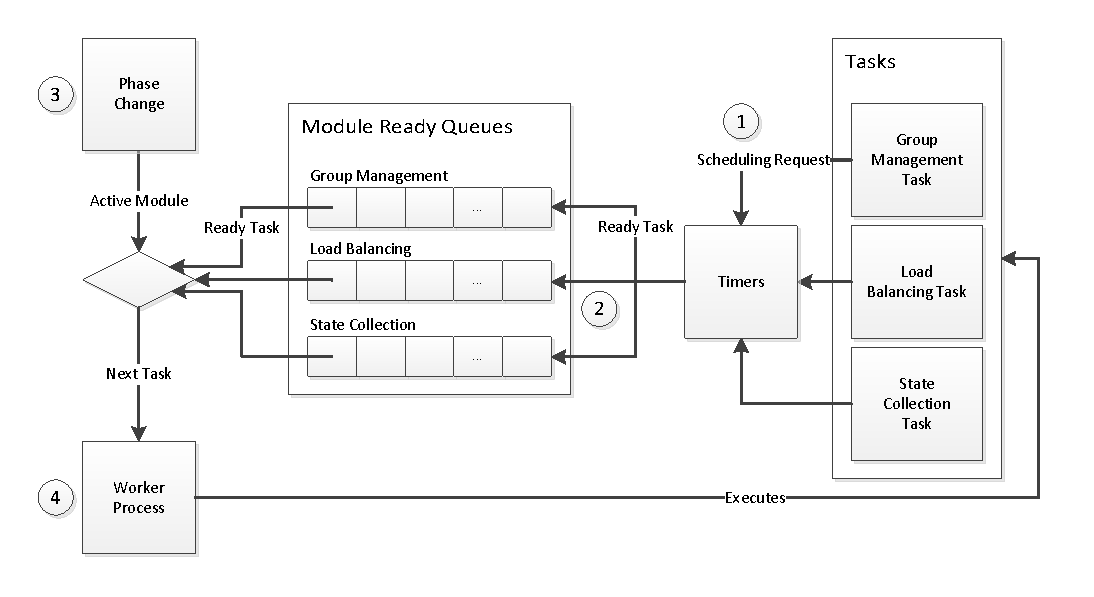
\includegraphics[width=1.0\textwidth]{RealTimeScheduler.pdf}
\captionsetup{singlelinecheck=off}
\caption[Real Time Scheduler]{The real time scheduler uses a round robin approach to allot execution time to modules. 
\begin{enumerate}
    \item Modules request that a task be executed by specifying a time in the
          future to execute a task. A timer is set to count down to the
          specified moment. Modules may also place tasks immediately into the
          ready queue if the task may be executed immediately.
    \item When the timer expires the task is placed into the ready queue for
          the module that requested the task be executed.
    \item Modules are assigned periods of execution (called phases) which are
          a predetermined length. After the specificed amount of time has
          passed, the module's phase ends and the next module in the schedule's
          tasks begin to execute.
    \item The worker selects the next ready task for the active module from the
          ready queue and executes it. These tasks may also schedule other tasks
          to be run in the future.
\end{enumerate}
}
\label{fig:REALTIMESCHEDULER}
\end{figure}

Modules inform the scheduler of tasks it wishes to perform by either submitting
them to be performed at some point in the future, or informing the scheduler of
a tasks that is ready to be executed immediately.

Tasks that have become ready, either by being inserted as ready, or the time
period that specified when it should be executed after has passed. The prepared
task is inserted into a ready queue for the module that the task has been
scheduled for.

When that modules phase is active, the task is pulled from the ready queue and
executed. When the phase is complete, the scheduler will stop pulling tasks
from the previous modules queue and begin pulling from the next modules queue.

This allows enforcement upper bound message delay. The modules have a specific
amount of processing time allotted. Modules with messages that invoke responses
(or a series of queries and responses) typically are required to be received
within the same phase, using round numbers which enforce that the message was
sent within the same phase.

Modules are designed and allotted time to allow for parameters such as maximum
query-response time (based on the latency between communicating processes). 
This implies that a module which engages in these activities has an
upper-bound in latency before messages are considered lost.

\section{Markov Models}

Markov models are a common way of recording probabilistic processes that can
be in various states which change over time. A Markov model is a directed
graph composed of states, and transitions between these states. Each
transition has some probability attached to them.

\subsection{Continuous Time Markov Chains}

The models begins in some initial state, and then transitions into other states
based on the probabilities assigned on each edge of the graph. Each state is
memoryless, meaning that the history of the system, or the previous states have
no effect on the next transition that occurs. Letting $Fx(s)$ equal the complete
history of a Markov chain $X$ up to time $s$, and letting $j \in S$, where $S$
is the complete set of states in the model. CITE STOICH BIO

\begin{equation}
P\{ X(t)=j | F_X(s) \} = P\{ X(t)=j | X(s) \}
\end{equation}

Additionally, the models we present are time homogeneous, meaning that the
time that transition probabilities are not affected by the amount of time that
has passed in the simulation. CITE STOICH BIO

\begin{equation}
P\{ X(t)=j | X(s) \} = P\{ X(t)=j | X(0) \}
\end{equation}

Models can be either discrete time or continuous time. In a discrete time model
time is divided into distinct slices. After each "slice" the system transitions
based on the random chance from each of possible transitions. The discrete model
also allows for a transition which returns to the same state.

To contrast, a continuous time model assumes that the time between transitions
are exponentially distributed. Each transition has some expected value or mean
value which describes the amount of time before a transition occurs. Continuous
time models do not have transitions which return to the same state since the
expected value of the transition time describes when how long the system 
remains in the same state The probability density
function (PDF) of the exponential distribution can be written as: CITE

\begin{equation}
f(x;\lambda) = \begin{cases}
\lambda e^{-\lambda x} & x \ge 0 \\
0, & x < 0
\end{cases}
\end{equation}

As a result, the expected or mean value of an exponential distribution, is a function of
the parameter $\lambda$: CITE

\begin{equation}
\mathrm{E}[X] = \frac{1}{\lambda}. \!
\end{equation}

When there are multiple possible transitions from a state, each with their own
expected transition time, the expected amount of time in the state is:

\begin{equation}
\sum \lambda(x,y) = \sum \lambda p_{x,y} = \sum \lambda(x)
\end{equation}

Where lambda(x,y) is the expected amount of time before state $x$ transitions to
state $y$. Interestingly, the expected time in a state ($\lambda(x)$) is related
to a the expected time for an individual transition ($\lambda(x,y)$) by a probability
$p_{x,y)$.

Each transition lends to an expected amount of time expected in the state. Then,
to do a random walk of a continuous time Markov chain, an intensity matrix must
also be generated in order to describe which transition is taken after the
exponentially distributed amount of time in the state has passed. Consider then
two streams of random variables, one of which is exponentially distributed and
used to determine the amount of time in a state. The second stream is normally
distributed and used to determine which state to transition to through the
intensity matrix.

\subsection{Modelling The Group}

To collect the in group time from a Markov model the SharpE tool was used.
Developed by Trivedi's team at Duke University, SharpE is a tool commonly used
for reliability and availability testing, and features a Markov chain tool. Data
collected from the simulator was used with SharpE to collect a steady state
probability (the probability that the system will be in a given state at any
given instant) from the collected simulation data.

Understanding how the dynamics of group formation is captured in a Markov Model 
is critical for both assessing its applicability and accuracy in this 
application. First, however, the dynamics of group membership must be 
understood as part of the distributed system.

Consider a set of processes, which are linked by some packet based network 
protocol. In our experiments we provide two protocols, each with different 
delivery characteristics. Under ideal conditions a packet sent by one process 
will always be delivered to its destination. Without a delivery protocol, as 
soon as packets are lost by the communication network, the message that it 
contained is lost forever. Therefore to compensate for the network losing 
packets, a large variety of delivery protocols have been adapted. Each protocol 
has a different set of goals and objectives, depending on the application.

Keeping in mind that a single lost packet does not necessitate the message it 
contained is forever lost, different protocols allow for different levels of 
reliability despite packet loss.

The leader election algorithm is centered around two critical events: checking, 
and elections. The check system is used to detect both failures and the 
availability of nodes for election.

Consider a set of processes which have already formed a group. These processes 
occasionally exchange messages to determine if the other processes have 
crashed. These processes can be classified into two sets: Leaders and Members.

\subsection{Failure Detection}

When a leader sends its check messages, the nodes that receive it either 
respond in the positive, indicating that they are also leaders, or in the 
negative indicating that they have already joined a group. This message is sent 
to all known nodes in the system. If a process replies that it is also a 
leader, the original sender will enter and election mode and attempt to combine 
groups with the first process. Nodes that fail to respond are removed from the 
leaders group, if they were members.

The member on the other hand will only direct its check message to the leader 
of its current group. As with the leader's check message, the response can 
either be positive or negative. A yes response indicates that the leader is 
still available and considers the member a part of its group. A no response 
indicates that either the leader has failed and recovered, or it has suspected 
the member process of being unreachable (either due to crash or network issue) 
and has removed them from the group. In this event the member will enter a 
recovery state and reset itself to an initial configuration where it is in a 
group by itself.

On any membership change, either due to recovery, or a suspected failure, the 
list of members for a group is pushed to every member of that group by the 
leader. Members cannot suspect other processes of being crashed, only the 
leader can identify failed group members.

\begin{figure}[!h]
\centering
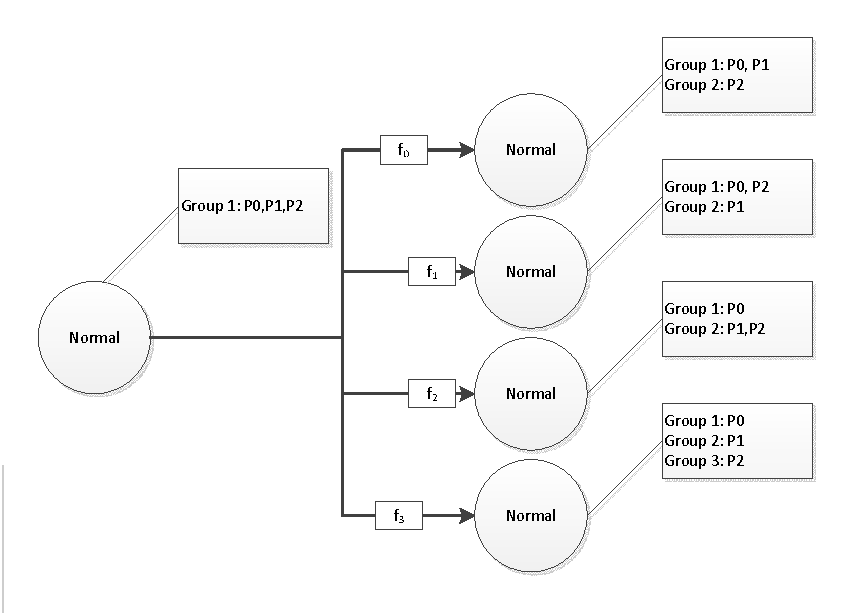
\includegraphics[width=1.0\textwidth]{markov-ayc.pdf}
\captionsetup{singlelinecheck=off}
\caption{A diagram showing a partial Markov chain for failure detection}
}
\label{fig:MARKOVAYC}
\end{figure}

A model of a failure detection stage of the leader election algorithm is presented in
Figure \ref{fig:MARKOVAYC}. A set of nodes begin in a normal state as part of a group.
The leader sends a query to every member, and every member sends a query to the leader.
If a response is not received in either direction, the process is considered to be 
unreachable and is either ejected from the group by the leader (if the query originated from the leader)
or the member leaves the group and becomes a coordinator themselves. 

The system will stay in the original state as long as all nodes complete their queries and responses.
Let $T_{RESPONSE}$ be the amount of time allowed for a response, $T_{BETWEENCHECKS} be the time between
discovery attempts, and $p_{FAILURE}$ is the probability that at least one peer fails to complete the exchange.
Based on this, the expected amount of time in the grouped state ($T_{GROUPED}) is:

\begin{equation}
\begin{cases}
T_{GROUPED} = ( T_{RESPONSE}+T_{BETWEENCHECKS}  ) / p_{FAILURE} & p_{FAILURE} > 0 \\
\infty & p_{FAILURE} = 0
\end{cases}
\end{equation}

Let $\delta$ equal exponential parameter of the exponential distribution for the base state. Then
we can relate the probabilities of each possible transition to the parameter for the base state. Let
$p_{i}$ be the probability of transitioning to configuration $i$ after leaving the base state and let
$f_{i}$ be the exponential parameter for the transition to an individual configuration:

\begin{equation}
$\delta = \sum f_{i} = \sum \delta p_{i} = \frac{1}{T_{GROUPED}}
\end{equation}

\subsection{Leader Election}

During elections, a highest priority leader (identified by its process id) will 
send invites to the other leaders it has identified. If those leaders accept 
the highest priority leader's invites, they will reply with an accept message 
and forward the invite to their members, if their are any. If the highest 
priority process fails to become the leader the next highest will send invites 
after a specified interval has passed.

Therefore, the membership of the system can be affected in two ways: election 
events which change the size of groups and failure suspicion (via checks) which 
decreases the size of groups. Note that elections can decrease the size of 
groups as well as increase them: If a round of forwarding invites fails by the 
new leader to his original group, the group size could decrease.

When a process is initialized it begins in the ``solo'' state: it is in a group 
with itself as the only member. As nodes are discovered by checks, the 
processes combine into groups. Groups are not limited by increasing one a time; 
they can increase by combined size of the groups of the leader processes.

We define a metric to assess the performance of the system under duress, we 
first consider that the distributed can only perform meaningful work when the 
processes can work together to perform physical migration. This means that 
there are two networks that affect the system's ability to do work: the 
physical and the cyber.

\begin{figure}[!h]
\centering
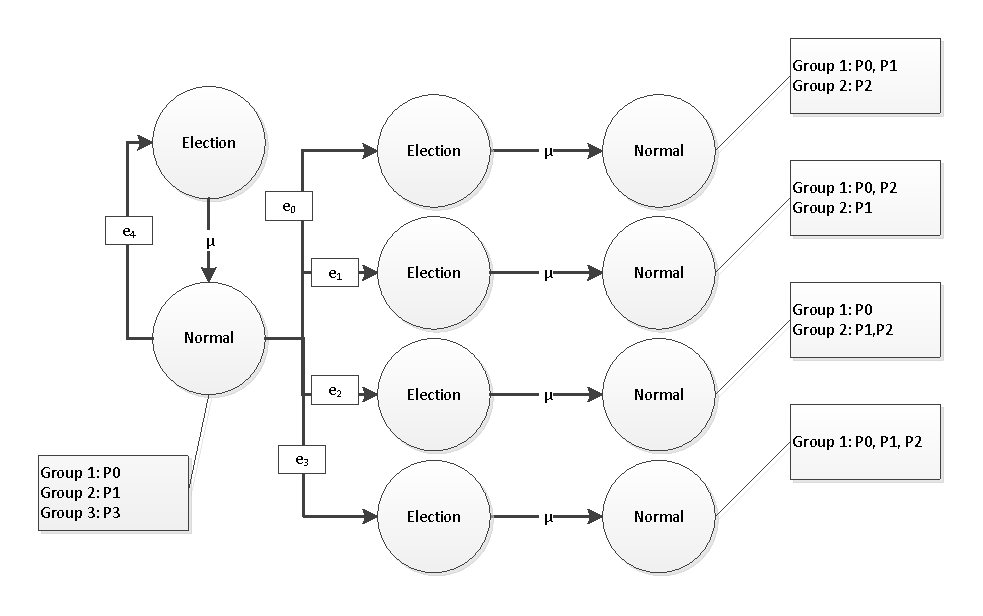
\includegraphics[width=1.0\textwidth]{markov-election.pdf}
\captionsetup{singlelinecheck=off}
\caption{A diagram showing a partial Markov chain for an election}
}
\label{fig:MARKOVELECTION}
\end{figure}

A continuous time Markov model of a single election is presented in Figure \ref{fig:MARKOVELECTION}.
A set of leaders begin in a normal state. After some time $T_{DISCOVER}$ an "are you coordinator"
message discovers some other other peer. $T_{DISCOVER}$ is a function of the number of discovery
checks which discover no leaders (which in turn is a function of the link reliability). Let
$T_{RESPONSE}$ be the amount of time allowed for a response, $T_{BETWEENCHECKS} be the time between
discovery attempts, and $p_{DISCOVERY}$ is the probability that the exchange discovers a leader.

\begin{equation}
\begin{cases}
T_{DISCOVER} = ( T_{RESPONSE}+T_{BETWEENCHECKS} ) / p_{DISCOVERY} & p_{DISCOVERY} > 0 \\
\infty & p_{DISCOVERY} = 0
\end{cases}
\end{equation}

Then, the parameter $\mu$ in Figure \ref{fig:MARKOVELECTION} is a function of $T_{DISCOVER}:

\begin{equation}
\mu = \frac{1}{T_{DISCOVER}}
\end{equation}

Once a leader has been discovered, the system transitions into an election state where the peers
hold an election to determine a new configuration. As shown in Figure \ref{fig: MARKOVELECTION},
an election can have a variety of outcomes. Each potential configuration is paired with an exponential distribution parameter
$e_{i}$ which is a function of the link reliability. The amount of time that an election takes is fixed
before the algorithm is executed. Let, $T_{ELECTION} be the mean time it takes to complete any election. Therefore:

\begin{equation}
\lamda = \sum e_{i} = \sum \lambda p_{i}
\end{equation}

Where $p_{i} is the probability (on transition) that the system transition to configuration $i$.

\subsection{Combined Model}

A combined model combines election and failure detection Markov chain components. Except for the
states where all reachable nodes are in the game group and the states where there are no reachable
leaders each state has a combination of an election transition and a failure transition. Given the
properties of continuous time distributions, let $\gamma_{X}$ equal the exponential parameter that
relates to the expected amount of time in a system configuration $X$. Then:

\begin{equation}
\gamma_{X} = \lambda_{X} = \delta_{X}
\end{equation}

Analysis of time in group is found as a steady state probability using SharpE. Analysis is done by
considering some node process $P_{i}$. If $P_{i}$ is a group with another process and not reconfiguring
that process contributes to the in-group steady state.